\documentclass[11pt,a4paper]{report}
\usepackage[utf8]{inputenc}
\usepackage[french]{babel}
\usepackage[T1]{fontenc}
\usepackage{amsmath}
\usepackage{amsfonts}
\usepackage{amssymb}
\usepackage{xcolor}

\usepackage{geometry}
\geometry{hmargin=2.5cm,vmargin=1.5cm}
\usepackage{wasysym}
\usepackage{graphicx}

\author{Mathieu Sarrat}
\title{LP4 - Modèle de l'écoulement parfait d'un fluide}

\makeatletter
\renewcommand{\thesection}{\@arabic\c@section}
\makeatother


\begin{document}
\maketitle

\section{Introduction}

Dans une leçon précédente nous avons discuté de la notion de viscosité (liée aux contraintes tangentielles exercées par un élément de fluide sur ses voisins) et établi l'équation modélisant le comportement d'un fluide visqueux (Navier-Stokes). Nous allons maintenant aborder un cas particulier important, celui où les effets de viscosité sont négligeables. Dans une telle situation, l'écoulement sera qualifié de parfait. 

\section{\'Ecoulement parfait d'un fluide}

\subsection{\'Ecoulement et fluide parfaits}

Un \textbf{fluide parfait} est un fluide dont la \textbf{viscosité dynamique $\eta $ est rigoureusement nulle}, ce qui est rare : l'hélium superfluide, à $T = 2.17 K$ est un exemple de fluide parfait. En général, il existe toujours une viscosité, aussi faible soit-elle.\\

On parler d'\textbf{écoulement parfait} lorsqu'on fait l'\textbf{approximation de négliger les effets liés à la viscosité}, et de façon générale, lorsqu'on omet tout effet susceptible de dissiper de l'énergie dans le fluide (diffusion, turbulence). L'évolution d'un fluide en écoulement parfait est donc une transformation adiabatique réversible, donc isentropique.\\

Cette approximation est applicable aux fluides réels dans plusieurs cas :
\begin{itemize}
	\item cas où les perturbations de $\bold{v}$ liées à la viscosité sont négligeables : écoulements dépendants du temps, échelles de temps courtes devant le temps de diffusion ou phénomènes de haute fréquence (phénomènes trop rapides pour laisser la diffusion agir)
	\item \'Ecoulements à grand nombre de Reynolds ($Re$) en dehors d'une zone appelée couche limite (région située entre le fluide parfait et une paroi), à condition qu'il n'y ait pas de turbulence (autre phénomène dissipatif).
\end{itemize}

\subsection{\'Equation d'Euler}

Reprenons l'équation de Navier-Stokes établie lors de la leçon précédente, dans le cas le plus général :
\begin{equation}
	\rho\left[\frac{\partial\bold{v}}{\partial t}+\left(\bold{v}\cdot\bold{\text{grad}}\right)\bold{v}\right]=\rho\bold{g}-\bold{\text{grad}}(p)+\eta\Delta\bold{v} 
	+ \left(\zeta + \frac{\eta}{3}\right)\bold{\text{grad}}\left(\text{div}\;\bold{v}\right) + \rho\bold{f},
\end{equation}
dont nous rappelons la signification des termes, de gauche à droite :
\begin{itemize}
	\item terme de non stationnarité de l'écoulement,
	\item terme de transport convectif,
	\item force volumique de pesanteur,
	\item force volumique de pression,
	\item force volumique de viscosité (diffusion),
	\item force volumique de viscosité liée aux variations de volume ($\zeta$ est la viscosité secondaire),
	\item forces volumiques occasionnelles, s'il y en a (à partir de maintenant, on décide qu'il n'y en a pas).
\end{itemize}

Cette équation est impossible à résoudre analytiquement telle quelle, d'où la nécessité de faire des approximations.\\

La première est \textcolor{red}{l'incompressibilité de l'écoulement} : $\text{div}\;\bold{v} = 0$, qui implique la constance de la masse volumique $\rho$ et la conservation du débit. Cette hypothèse est valable tant que la vitesse maximale de l'écoulement reste suffisamment petite devant la célérité du son dans le fluide.\\

Si un fluide est parfait, on pose $\eta = 0$ et $\zeta = 0$ pour obtenir l'\textcolor{red}{\textbf{équation d'Euler}}
\begin{equation}
	\rho\frac{\partial\bold{v}}{\partial t}+\left(\bold{v}\cdot\bold{\text{grad}}\right)\bold{v}=\rho\bold{g}-\bold{\text{grad}}(p).
\end{equation} 
Bien que les fluides parfaits soient rares, on peut faire l'hypothèse d'un écoulement parfait, auquel cas l'équation d'Euler devient une approximation, dont nous allons discuter la validité.

Nous avons introduit le nombre de Reynolds comme une mesure du rapport :
\begin{equation}
	Re = \frac{U L}{\nu} \simeq \frac{|\rho \left(\bold{v}\cdot\textbf{grad} \right) \bold{v}|}{|\eta \Delta \bold{v}|},	
\end{equation}
où $U$ et $L$ sont la vitesse caractéristique de l'écoulement et la longueur de variation typique du profil de vitesse.

Rigoureusement, l'équation d'Euler est valable pour un nombre de Reynolds infini.

En pratique, on peut l'utiliser pour un grand nombre de Reynolds tant qu'on reste \textbf{loin des bords} (hors de la couche limite) \textbf{et} qu'il n'y a \textbf{pas de turbulence} (on veut un régime laminaire, soit $Re < 2000$. Au-delà le régime est turbulent et une description plus détaillée est nécessaire.

A faible nombre de Reynolds, on ne peut pas négliger le terme diffusif, qui est prédominant. Il est possible malgré tout d'utiliser l'équation d'Euler si le phénomène étudié est très rapide devant le temps caractéristique du transport diffusif, donné par $\tau \sim L^2/\nu$.  

\subsubsection{Remarque 1 : équations et inconnues}
Cette équation vectorielle conduit à trois équations scalaires, pour cinq inconnues ($\rho$, les trois composantes de la vitesse et $p$). 
Deux équations supplémentaires sont donc nécessaires : l'équation de continuité 
\begin{equation}
	\frac{\partial \rho}{\partial t} + \text{div}\;\left(\rho\bold{v}\right) = 0
\end{equation}
et une relation de fermeture (car elle ferme le système d'équations) qui peut être une équation d'état thermodynamique. 

L'hypothèse d'un écoulement incompressible permet de réécrire l'équation de continuité
\begin{equation}
	\frac{\partial \rho}{\partial t} + \left(\bold{v}\cdot\textbf{grad}\right)\rho = \frac{d\rho}{dt} = 0.
\end{equation} 
La masse volumique d'une particule fluide reste donc constante au cours du temps (point de vue Lagrangien). Le fait de supposer un écoulement stationnaire force la masse volumique à être homogène : $\rho = \text{cte}$.\\

Concernant la relation de fermeture, l'hypothèse qui est souvent faite est de considérer un écoulement \textcolor{red}{barotrope}, pour lequel la pression ne dépend que de la masse volumique, ce qui ôte bien une variable du problème.

\subsubsection{Remarque 2 : conditions aux limites et notion de couche limite}

Les conditions aux limites sont nécessaires pour déterminer les constantes qui apparaissent inévitablement lors de la résolution de l'équation d'Euler.\\

\begin{itemize}
	\item \textcolor{red}{Contact fluide/solide :}\\
	\begin{itemize}
		\item paroi imperméable, donc $v_{\text{solide}}\cdot\bold{n} = v_{\text{fluide}}\cdot\bold{n}$ : 
			égalité de la composante normale de la vitesse à l'interface, qui est nulle si la paroi est au repos
		\item tangentiellement, \textbf{le fluide peut glisser parallèlement à la paroi} : il n'y a donc pas de condition sur la composante tangentielle\\
	\end{itemize}

	\item \textcolor{red}{Contact entre deux fluides :}\\
	En plus de la contrainte sur les vitesses présentée ci-dessus (valable pour une interface fluide/fluide), 
	il faut ajouter une \textcolor{red}{condition sur les contraintes normales et tangentielles} à l'interface.\\
	
	Pour une interface de forme quelconque, le problème est un peu plus complexe et fait intervenir la notion de tension de surface, qui sera abordée dans une autre leçon.
	Néanmoins, \textbf{si l'interface entre les deux fluides est plane}, les choses sont plus simples :
	\begin{itemize}
		\item \textbf{égalité des pressions} (contraintes normales) : $p_{\text{fluide}\;1} = p_{\text{fluide}\;2}$
		\item l'un des deux fluides étant parfait, les contraintes tangentielles à l'interface sont nulles;
	\end{itemize}
\end{itemize}

Ce modèle ne correspond pas à la réalité physique. Même si le nombre de Reynolds est fort, un écoulement n'est jamais parfait à proximité d'une interface, région où les phénomènes de viscosité sont présents et permettent d'assurer adhérence et frottements.\\

Considérons un objet de taille $L$ se déplaçant à une vitesse $U$. \'A l’instant $0$ l’extrémité du système est en O. 
\'A l’instant $t$ tout le corps s’est déplacé tel qu’en O on ait l’autre extrémité de l’objet. Le frottement visqueux de l'objet dans le fluide est modélisé par une force de traînée. Il s’est créé en O toute une couche (appelée \textbf{couche limite}) où le transport de la quantité de mouvement (transmise au fluide du fait de la viscosité de ce dernier et du déplacement de l'objet) se produit. Cette couche a une épaisseur $\delta$ donnée par la longueur caractéristique de diffusion (Figure \ref{fig:couche_limite}).

\begin{figure}[h!]
\begin{center}
	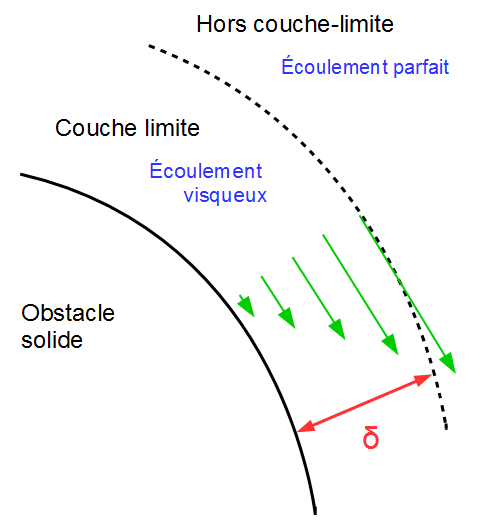
\includegraphics[scale = 0.3]{couche_limite.png}
	\caption{Schéma d'une couche limite, pour un écoulement à fort nombre de Reynolds}. 
	\label{fig:couche_limite}
\end{center}
\end{figure}

Ainsi, en assimilant le temps de diffusion à la durée de déplacement de l'objet $t$ :
\begin{equation}
	\delta \sim \sqrt{\nu t}.
\end{equation}
Comme $Re = UL/\nu$ (donc $\nu = UL/Re$) et $U = L/t$, on obtient
\begin{equation}
	\delta \sim \frac{L}{\sqrt{Re}}
\end{equation}
Remarquons que pour un fluide parfait, $Re \rightarrow \infty$, donc $\delta \rightarrow 0$ : on retrouve bien ce qu'on disait plus haut.

Pour pouvoir considérer un écoulement comme parfait il faudra donc se placer à une distance $d \gg \delta$ (avec $\delta \ll L$, sans quoi l'écoulement est rampant et la viscosité domine) de l’interface.\\

L’existence de la couche limite permet par exemple de comprendre le sillage formé par un avion en déplacement dans l'air. Loin de l'avion, l'écoulement de l'air peut être vu comme parfait. En ordre de grandeur, nous pouvons dire qu’un nageur (taille de $1m$) nageant à $1m/s$ dans l’eau, ou une voiture allant à $90km/h$ dans l’air correspondent à des écoulements parfaits (grand Reynolds et $\delta \sim 1$ mm). Par contre, le mouvement d'une bactérie dans l'eau (taille $100 \mu m$, vitesse 30 $\mu m/s$) correspond à un écoulement rampant ($Re\sim 10^{-3}$, $\delta \sim 500 \mu m \sim L$), non modélisable comme un écoulement parfait. 

\subsubsection{Remarque 3 : nombres sans dimension et similitudes (facultatif)}

La résolution de l'équation d'Euler est complexe, du fait du terme convectif, non-linéaire. L'utilisation de nombres sans dimension permettant de comparer l'importance relative de deux termes figurant dans l'équation permet de la simplifier en négligeant les effets négligeables au vu de la géométrie de l'écoulement.\\

Le nombre de Reynolds est l'un de ces nombres, mais il en existe d'autres. Citons par exemple
\begin{itemize}
	\item le \textcolor{red}{nombre d'Euler $Eu$ :}
	\begin{equation}
		\displaystyle{Eu \equiv \frac{p}{\rho U^2} \simeq \frac{|\textbf{grad}\;p|}{|\rho\left(\frac{\partial \bold{v}}{\partial t} 
		+ \left(\bold{v}\cdot\textbf{grad}\right)\right)\bold{v}|}}
	\end{equation}
	On peut négliger les forces de pression si $Eu$ est faible.
	\item le \textcolor{red}{nombre de Froude $Fr$ :}
	\begin{equation}
		\displaystyle{Fr \equiv \frac{|\rho\left(\frac{\partial \bold{v}}{\partial t} 
		+ \left(\bold{v}\cdot\textbf{grad}\right)\right)\bold{v}|}{|\rho \bold{g}|}}
	\end{equation}
	Si $Fr$ est grand, on peut négliger l'influence de la pesanteur.\\
\end{itemize}

La similitude est la mise en évidence de nombres sans dimensions permettant de réduire le nombre de paramètres intervenant dans les équations décrivant un système afin de simplifier son analyse, voire ses équations comme dans le cas de la couche limite. Cela permet la définition d'expériences représentatives à une échelle plus accessible que le phénomène réel.

Exemple : si on adimensionne Navier-Stokes incompressible, on fait apparaître les nombres de Reynolds et de Froude. Deux problèmes différents, obéissant à cette même équation et dont les nombres $Re$ et $Fr$ sont similaires et on s'attend à observer expérimentalement le même comportement : maquettes...

\subsubsection{Remarque 4 : réversibilité}

Cette équation est invariante par renversement du temps, impliquant la réversibilité des phénomènes qu'elle décrit.

\section{Aspects énergétiques}

\subsection{Relations de Bernoulli}
Il est possible de décrire un fluide parfait par une approche "différente" mais équivalente à la résolution de l'équation d'Euler. Il s'agît de transformer l'équation d'Euler pour faire apparaître un bilan énergétique. Prenons pour cela l'équation d'Euler :

\begin{equation}
	\rho\left(\frac{\partial\bold{v}}{\partial t}+\left(\bold{v}\cdot\textbf{grad}\right)\bold{v}\right)=\rho\bold{g}-\bold{\text{grad}}(p),
\end{equation}
et utilisons l'égalité suivante
\begin{equation}
	\left(\bold{v}\cdot\textbf{grad}\right)\bold{v} = \frac{1}{2}\textbf{grad}\;v^2 + \textbf{rot}\;\bold{v}\times\bold{v}.
\end{equation}
On obtient
\begin{equation}
	\frac{\partial\bold{v}}{\partial t} +  \textbf{grad}\left(\frac{v^2}{2}\right) + \textbf{rot}\;\bold{v}\times\bold{v}
	= - \frac{1}{\rho}\textbf{grad}\;p + \bold{g}.
\end{equation}

Supposons un \textbf{écoulement stationnaire}, et faisons le produit scalaire de l'équation par $d\bold{r} = \bold{v}(\bold{r},t)dt$, 
déplacement élémentaire d'une particule fluide le long de sa trajectoire dans l'écoulement (ce n'est pas un déplacement virtuel, et comme l'écoulement est stationnaire, ligne de courant et trajectoires sont confondues) :
\begin{equation}
	\underbrace{\textbf{grad}\left(\frac{v^2}{2}\right)\cdot d\bold{r}}_{=d(v^2/2)} 
	+ \underbrace{\left(\textbf{rot}\;\bold{v}\times\bold{v}\right)\cdot d\bold{r}}_{= \bold{0}}
	= - \frac{1}{\rho}\underbrace{\textbf{grad}\;p\cdot d\bold{r}}_{= dp} 
	+ \underbrace{\bold{g}\cdot d\bold{r}}_{= d\left(\bold{g}\cdot\bold{r}\right)}.
\end{equation}
d'où
\begin{equation}
	\frac{v^2}{2} -\bold{g}\cdot\bold{r} + \int\frac{dp}{\rho} = \text{Cte}.
\end{equation}
On a \textbf{intégré l'équation d'Euler sur une ligne de courant/trajectoire de particule fluide} : c'est une intégrale première du mouvement. 
\textcolor{red}{Faire un schéma.}\\

\textbf{Remarque :} dans un écoulement irrotationnel (vorticité nulle), caractérisé par
\begin{equation}
	\textbf{rot}\;\bold{v} = 0,
\end{equation}
(également appelé écoulement potentiel car dans ce cas $\bold{v} = \textbf{grad}\;\Phi$) l'équation de Bernouilli est valable sur n'importe quelle courbe à l'intérieur du fluide, puisque pour annuler
\begin{equation}
	\left(\textbf{rot}\;\bold{v}\times\bold{v}\right)\cdot d\bold{r}
\end{equation}
on n'a plus besoin que le déplacement $d\bold{r}$ suive une trajectoire réelle (i.e. vérifie $d\bold{r} = \bold{v}(\bold{r},t)dt$).

\subsubsection{Relation de Bernoulli pour un écoulement incompressible}

Si nous faisons l'hypothèse d'un \textbf{écoulement incompressible} ($\rho$ indépendante du temps, et de l'espace car régime stationnaire) 
\begin{equation}
	\frac{v^2}{2} -\bold{g}\cdot\bold{r} + \frac{p}{\rho} = \text{Cte}.
\end{equation}
le long d'une ligne de courant/trajectoire (et seulement dans ce cas).

Si on prend $z$ comme direction pour la verticale (axe orienté vers le haut),
\begin{equation}
	\frac{v^2}{2} + gz + \frac{p}{\rho} = \text{Cte}.
\end{equation}
Ce résultat n'est valable que le long d'une trajectoire de particule fluide (et donc le long d'une ligne de courant, seulement car le régime est stationnaire).
 
\subsubsection{Relation de Bernoulli pour un écoulement barotrope}

Si nous faisons l'hypothèse d'un \textbf{écoulement barotrope} ($p = f(\rho)$ et donc $\rho = f(p)$),
on peut écrire 
\begin{equation}
	\frac{dp}{\rho} \equiv df(p),
\end{equation}
où $f$ est une fonction de la pression seulement.

Dans ce cas, la relation de Bernoulli devient
\begin{equation}
	\frac{v^2}{2} + gz + f(p) = \text{Cte}.
\end{equation}
Encore une fois, ce résultat n'est valable que le long d'une trajectoire de particule fluide (et donc le long d'une ligne de courant, seulement car le régime est stationnaire).\\

\textbf{Exemples} pour $f(p)$ (facultatif):
\begin{itemize}
	\item \textcolor{red}{gaz parfait et évolution isotherme (réalisme, le fluide était parfait ??)}
	\begin{equation}
		pV = nRT \Rightarrow \rho = \frac{Mp}{RT}
	\end{equation}
	où $M$ est la masse molaire du gaz. Dans ce cas
	\begin{equation}
		f(p) = \int \frac{dp}{\rho} = \frac{RT}{M}\int \frac{dp}{p} = \frac{RT}{M}\text{ln}\;p + \text{Cte},
	\end{equation}
	d'où Bernoulli :
	\begin{equation}
		\frac{v^2}{2} + gz + \frac{RT}{M}\text{ln}\;p = \text{Cte}.\\
	\end{equation}
	
	\item \textcolor{red}{gaz parfait et évolution adiabatique réversible (préférable car fluide parfait)}\\
	On a $pV^{\gamma} = \text{Cte}$, d'où $p/\rho^\gamma = K$, $K$ constante. D'où $\rho = p^{1/\gamma}K^{-1/\gamma}$. Rappelons que $\gamma$ est le rapport des capacités thermiques à pression et à volume constants. 
	\begin{equation}
		\frac{dp}{\rho} = K^{1/\gamma} p^{-1/\gamma} dp = d\left(K^{1/\gamma}\frac{p^{1-\frac{1}{\gamma}}}{1-\frac{1}{\gamma}}\right)
	\end{equation}
	d'où Bernoulli
	\begin{equation}
		\frac{v^2}{2} + gz + K^{1/\gamma}\frac{p^{1-\frac{1}{\gamma}}}{1-\frac{1}{\gamma}} = \text{Cte}.
	\end{equation}
\end{itemize}


\subsection{Interprétation énergétique des relations de Bernoulli}

La relation de Bernoulli traduit un bilan d'énergie cinétique pour une particule fluide tout au long de son mouvement. Elle traduit la conservation de l'énergie dans un écoulement parfait.

\textcolor{red}{Démonstration : facultative}

\begin{figure}[h!]
\begin{center}
	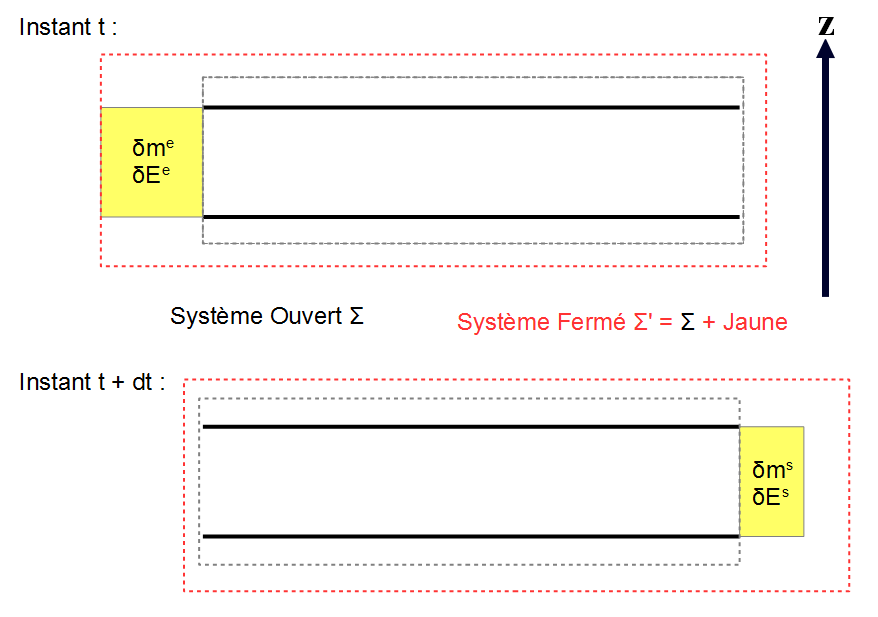
\includegraphics[scale = 0.3]{bilan_bernoulli.png}
	\caption{Interprétation énergétique des relations de Bernoulli}. 
	\label{fig:bilan_bernoulli}
\end{center}
\end{figure}

Illustrons ceci en effectuant un bilan d'énergie sur le système représenté en figure \ref{fig:bilan_bernoulli}.

Soit le système fermé $\Sigma'$ constitué par une quantité de fluide donnée, donc de masse $m'$ invariante dans le temps, et d'énergie totale $E'$ (dont la variation obéit au Premier Principe de la Thermodynamique). \textit{On n'a pas $E'(t+dt) = E'(t)$ car $E'$ est une quantité Lagrangienne, contrairement à $E$ qui est Eulérienne (et donc invariante si le régime est stationnaire).}\\

\'A l'instant $t$, la masse $m'$ est partiellement contenue dans le sous-système ouvert $\Sigma$ : une quantité de masse $\delta m^e$, de vitesse $v_e$ et d'énergie 
\begin{equation}
	\delta E^e = \frac{1}{2}\delta m^e v_e^2 + \delta m^e u_e + \delta m^e g z_e
\end{equation}
(où $u_e$ est l'énergie interne massique de cette quantité de fluide) n'est pas encore entrée dans $\Sigma$. On note $m(t)$ la masse contenue par $\Sigma$ à l'instant $t$.

\'A l'instant $t+dt$, le système $\Sigma$ contient la masse $m(t+dt)$. Une quantité de masse $\delta m_s$, de vitesse $v_s$ et d'énergie $\delta E^s$ est sortie de $\Sigma$ de sorte que $M(t+dt) = m(t) + \delta E^s$.\\

\textcolor{red}{Bilan de masse :}
\begin{equation}
	m'(t) = m(t) + \delta m^e = m'(t+dt) = m(t+dt) + \delta m^s \Rightarrow m(t+dt) - m(t) \equiv \frac{\partial m}{\partial t}dt = \delta m^e - \delta m^s.
\end{equation}
puisque $m'(t+dt) = m(t)$ (système $\Sigma'$ fermé). 
En supposant un \textcolor{red}{régime stationnaire, $\partial m/\partial t = 0$, d'où $\delta m^e = \delta m^s \equiv \delta m$.}\\

\textcolor{red}{Bilan d'énergie :}
\begin{equation}
	E'(t) = E(t) + \delta E^e
\end{equation}
et 
\begin{equation}
    E'(t+dt) =  E(t+dt) + \delta E^s.
\end{equation}
Donc
\begin{equation}
	E'(t+dt) - E'(t) = \frac{\partial E}{\partial t}dt + \delta E^s - \delta E^e.
\end{equation}
En régime stationnaire ($\partial E/\partial t = 0$ et $\delta m^e = \delta m^s \equiv \delta m$), donc
\begin{equation}
	E'(t+dt) - E'(t) = \delta E^s - \delta E^e = \delta m \left[\frac{1}{2}\left(v_s^2 - v_e^2\right) + u_s - u_e + g\left(z_s - z_e\right)\right].
\end{equation}
\begin{equation}
	E'(t+dt) - E'(t) = \delta m {\left[\frac{v^2}{2} + u + gz\right]^s}_e.
\end{equation}

Par application du Premier Principe, on a aussi
\begin{equation}
	E'(t+dt) - E'(t) = \delta W_p + \delta W_u + \delta Q,
\end{equation}
où on a distingué le travail des forces de pression $\delta W_p$ de celui des autres forces $\delta W_u$ (par exemple celui d'une pompe).

Ainsi
\begin{equation}
	\delta m {\left[\frac{v^2}{2} + u + gz\right]^s}_e = \delta W_p + \delta W_u + \delta Q.
\end{equation}

L'écoulement étant supposé incompressible on peut supposer $u$ constante. En l'absence de viscosité et de source d'énergie extérieure, $\delta W_u$ et $\delta Q$ sont nuls.
En supposant un écoulement adiabatique réversible, \textcolor{red}{$\delta W_p = p_e dV_e - p_s dV_s$}, d'où
\begin{equation}
	\delta m {\left[\frac{v^2}{2} + gz + \frac{p}{\rho}\right]^s}_e = 0,
\end{equation}
qui est bien la relation de Bernoulli.

\section{Applications}

\subsection{Effet Venturi}

L'effet Venturi désigne la formation d'une dépression au niveau du rétrécissement d'un tube. On peut expliquer cet effet très simplement, à partir de la relation de Bernoulli et de l'incompressibilité du fluide. Considérons le système représenté en figure \ref{fig:venturi} \textcolor{red}{(sans les tubes manométriques pour commencer)}, en régime stationnaire.
\begin{figure}[h!]
\begin{center}
	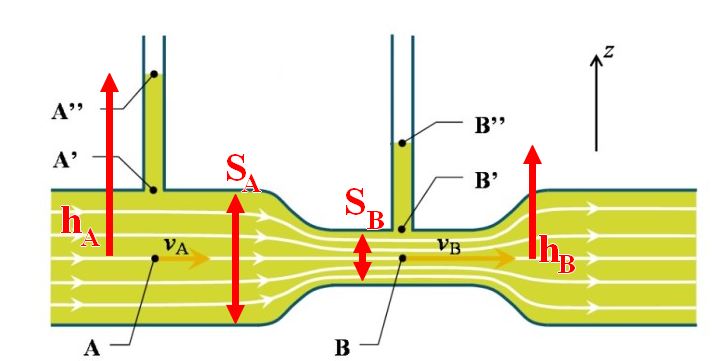
\includegraphics[scale = 0.3]{venturi.png}
	\caption{Tube de Venturi.} 
	\label{fig:venturi}
\end{center}
\end{figure}

L'incompressibilité implique la conservation du débit :
\begin{equation}
	v_A S_A = v_B S_B;
\end{equation}
on voit bien qu'un rétrécissement du conduit entraîne une augmentation de la vitesse du fluide. 

Appliquons la relation de Bernoulli à la ligne de courant $AB$ :
\begin{equation}
	p_A + \frac{\rho v_A^2}{2} + \rho g z_A = p_B + \frac{\rho v_B^2}{2} + \rho g z_B. 
\end{equation}
Les termes de pesanteur sont égaux ($z_A = z_B$), il ne reste donc que :
\begin{equation}
	p_A - p_B = \frac{\rho}{2}\left(v_B^2 - v_A^2\right) = \frac{\rho v_B^2}{2}\left(1 - \frac{S_B^2}{S_A^2}\right) > 0.
\end{equation}

On constate que $p_B$ est plus faible que $p_A$ : c'est l'effet Venturi.

\subsubsection{Filtration sous vide}
	\begin{figure}[h!]
	\begin{center}
		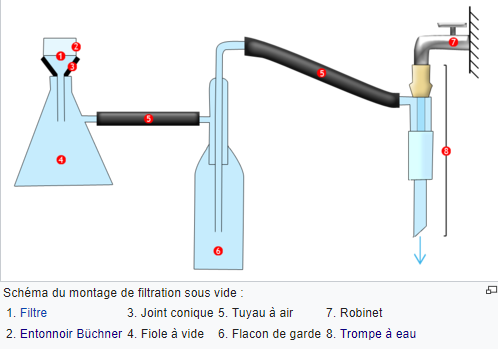
\includegraphics[scale = 0.5]{filtration_vide.png}
		\caption{Dispositif de filtration sous vide.} 
		\label{fig:filtration_vide}
	\end{center}
	\end{figure}

\textcolor{red}{Utilisations :}
\begin{itemize}
	\item séparer un solide d'un liquide (isoler un solide en suspension après production)
	\item purifier un liquide s'il contient des contaminants solides
\end{itemize}

\textcolor{red}{Principe :}
\begin{itemize}
	\item L'eau s'écoule dans la trompe à eau : aspiration de l'air contenu dans le flacon de garde et dans la fiole à vide (par effet Venturi).
	\item Différence de pression entre l'extérieur et l'intérieur des fioles : le contenu de l'entonnoir Büchner est aspiré vers la fiole à vide.
	\item Le filtre posé dans le fond de l'entonnoir Büchner sépare le solide du liquide.
	\item Le solide (résidu de filtration), qui reste dans le haut de l'entonnoir Büchner, est alors récupéré (plus sec qu'avec filtration simple)
\end{itemize}

\textcolor{red}{Remarques :}
\begin{itemize}
	\item La filtration est aussi une étape de purification : les impuretés solubles dans le solvant sont éliminées dans le filtrat (liquide)
	\item Joint conique : assure l'étanchéité du montage (empêche le passage de l'air entre l'entonnoir Büchner et la fiole à vide).
	\item Montage aussi utilisé pour purifier un liquide : les insolubles (catalyseurs, impuretés, sous-produits de réaction, sels…) sont retenus sur le filtre.
	\item Montage instable : maintenir la fiole à vide et le flacon de garde (pinces). 
	\item Avant de fermer le robinet, il est nécessaire de "casser le vide" (on enlève l'entonnoir), sinon de l'eau remonte par la trompe à eau. 
	Sinon, le flacon de garde empêche l'eau de remonter dans la fiole à vide.
\end{itemize}

\subsubsection{Mesure du débit d'une canalisation}
	
	On introduit deux tubes manométriques pour mesurer la pression aux points A et B : l'ensemble constitue un tube de Venturi (deux sections de canalisation et un étranglement au milieu). L'eau va monter jusqu'à une certaine hauteur, différente dans chacun des deux tubes (on note ces hauteurs $h_A$ et $h_B$). La connaissance de la hauteur d'eau permet de remonter à la différence de pression $p_A - p_B$ et donc au débit d'eau.\\	
	
	L'instrument de mesure ne doit pas perturber le système. Tout comme un voltmètre ne doit laisser passer que très peu de courant pour mesurer une différence de potentiel sans perturber le circuit sur lequel il est connecté en dérivation, il ne doit pas y avoir de courant (i.e. d'écoulement) dans les tubes manométriques. La section de ces tubes doit donc être suffisamment petite. Dans ce cas :
	\begin{itemize}
		\item écoulement peu perturbé et donc uni-directionnel dans la conduite (prises de pression loin des régions où la section de la conduite varie !). 
		Gradient vertical de pression entre A et A' (resp. entre B et B') hydrostatique;
		\item pas d'écoulement dans les tubes, donc \textcolor{red}{gradient vertical de pression hydrostatique} entre A' et A'' (resp. entre B' et B'');\\
	\end{itemize}

La surface libre de l'eau dans les tubes est au contact de l'air ambiant, donc $p_A'' = p_B'' = p_0$. D'où :
\begin{equation}
	p_A = p_0 + \rho g h_A
\end{equation}
et
\begin{equation}
	p_B = p_0 + \rho g h_B.
\end{equation}

	\begin{itemize}
		\item Bernoulli : $h_B < h_A$
		\item Bernoulli : expression du débit (calcul ci-dessous)
	\end{itemize}

\begin{equation}
	p_A - p_B \equiv \Delta p = \rho g \underbrace{\left(h_A - h_B\right)}_{\Delta h} = \rho g \Delta h = \frac{\rho v_B^2}{2}\left(1 - \frac{S_B^2}{S_A^2}\right)
\end{equation}
D'où le débit :
\begin{equation}
	D_m = \rho S_B S_A \sqrt{\frac{2g\Delta h}{S_A^2 - S_B^2}} = S_A S_B \sqrt{\frac{2\rho \Delta p}{S_A^2 - S_B^2}}.
\end{equation}

\subsection{Théorème de Torricelli}
\begin{figure}[h!]
\begin{center}
	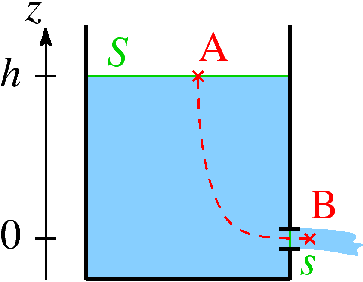
\includegraphics[scale = 0.3]{torricelli.png}
	\caption{Démonstration du théorème de Torricelli}. 
	\label{fig:torricelli}
\end{center}
\end{figure}

Soit une citerne remplie d'eau \ref{fig:torricelli}. On perce un orifice à une hauteur choisie comme niveau de référence. On repère son niveau par la hauteur $h$. La section  de l'orifice est notée $s$, la section de la citerne est $S$.\\

\textcolor{red}{Hypothèses :}
\begin{itemize}
	\item écoulement parfait,
	\item écoulement incompressible,
	\item régime stationnaire (bonne approximation si $S >> s$).
\end{itemize}

On applique la relation de Bernoulli à la ligne de courant $AB$. Du fait de l'égalité des pressions aux points A et B (pression atmosphérique) :
\begin{equation}
	\frac{\rho v_A^2}{2} + \rho g z_A = \frac{\rho v_B^2}{2} + \rho g z_B.
\end{equation}

Le régime stationnaire implique la conservation du débit,
\begin{equation}
	\rho v_A S = \rho v_B s,
\end{equation}
d'où, en injectant dans Bernoulli,
\begin{equation}
	v_B = \sqrt{\frac{2gh}{1 - s^2/S^2}}.
\end{equation}

Si $s << S$, $v_B \simeq \sqrt{2gh}$, soit la vitesse qu'aurait acquise la particule de fluide après une chute libre de hauteur $h$.

\subsection{Effet de courbure}
Soit un écoulement parfait dont les lignes de courant sont courbes. On suppose que les forces volumiques, telles que la pesanteur, sont négligeables.\\

L'équation d'Euler devient :
\begin{equation}
	\rho \frac{d\bold{v}}{dt} = - \textbf{grad}\;p
\end{equation}
Soit $\bold{e}_t$ et $\bold{e}_n$ les vecteurs unitaires tangent et normal à une ligne de courant ($\bold{v} = v\bold{t}$). L'équation d'Euler s'écrit :
\begin{equation}
	\rho \frac{d\bold{v}}{dt} = \rho \frac{dv}{dt}\bold{t} + \rho v \frac{d\bold{t}}{ds}\frac{ds}{dt} =\rho \frac{dv}{dt}\bold{t} + \rho \frac{v^2}{R}\bold{n} = -\textbf{grad}\;p
\end{equation}
où $s$ est l'abscisse curviligne le long d'une ligne de courant et R le rayon de courbure local de la ligne.\\

On projette l'équation d'Euler selon ces deux vecteurs, d'où
\begin{equation}
	\rho \frac{dv}{dt} = -\frac{\partial p}{\partial \bold{r}}\cdot\bold{t} = - \frac{\partial p}{\partial s}
\end{equation}
et
\begin{equation}
	\frac{\rho v^2}{R} = -\frac{\partial p}{\partial \bold{r}}\cdot\bold{n} > 0.
\end{equation}
 
Il découle de cette dernière équation que
\begin{equation}
	\frac{\partial p}{\partial \bold{r}}\cdot\bold{n} < 0,
\end{equation}
et donc que la pression diminue lorsqu'on se rapproche du centre de courbure de la ligne de courant. Elle augmente lorsqu'on s'en éloigne.\\

Ce phénomène est à la base de l'effet Coanda. L'effet Coanda est la tendance d'un écoulement de gaz à être attiré par une surface convexe que l'on approche de lui (avec l'eau, on parle d'effet théière et les causes du phénomène sont différentes). Ainsi, un jet d'air originellement rectiligne sera dévié si on place un obstacle cylindrique perpendiculairement à sa direction au-dessous de lui. Le jet épousera la surface de l'objet sur une certaine longueur. La force résultant de la différence de pression liée à la courbure (et qui correspond à la variation temporelle de la quantité de mouvement du jet due à sa déviation) est ainsi capable de maintenir en "lévitation" apparente une balle de ping pong. Il faut bien entendu pour cela qu'elle compense le poids et la force d'entraînement par la viscosité exercée par le jet sur la balle.

	\begin{figure}[h!]
	\begin{center}
		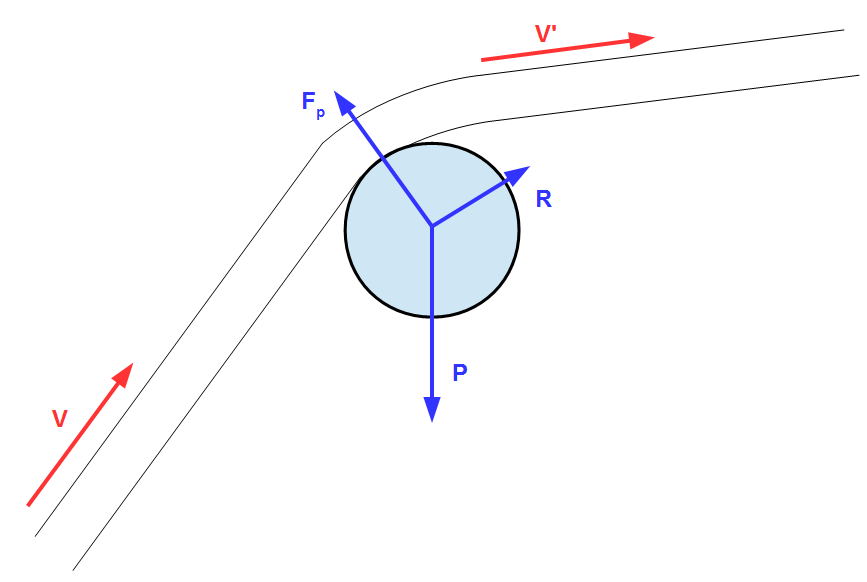
\includegraphics[scale = 0.5]{coanda.png}
		\caption{Dispositif de filtration sous vide.} 
		\label{fig:coanda.png}
	\end{center}
	\end{figure}

\newpage
\section{Conclusion}

Le modèle de l'écoulement parfait d'un fluide est une approximation consistant à ignorer les effets dissipatifs (liés à la viscosité, ou à la turbulence). Cette approximation est tout à fait valable en dehors de la région faisant interface entre une paroi et le fluide, appelée couche limite. L'épaisseur de cette couche est d'autant plus faible que la vitesse caractéristique de l'écoulement est importante et que le fluide est peu visqueux. De tels écoulements correspondent à un nombre de Reynolds élevé. Le modèle de l'écoulement parfait n'est pas utilisable en présence de turbulence.



\end{document}